\chapter{Implementation}
\label{sec:implementation}
\index{CRAVA!implementation}


NBNB Ragnar: Skriv denne biten p� nytt.

\section{Using fft for inversion}
\section{Local wavelet and noise}
\section{Estimation of parameters}
\subsection{Estimating wavelet and noise}
\subsection{Estimating correlations}
\subsection{Estimating background model}

The \crava program gives an efficient implementation of the posterior
distribution given in equations \eqref{mu_post} and
\eqref{Sigma_post}, both in terms of computation and storage.

As prior information\index{prior model}, \crava estimates the
expectations $\bmu_m$, the correlation matrix $\bSigma_{0,m}$, and the
temporal correlation function $\cmt(\tau)$ directly from well
data. The lateral correlation functions $\cml(\xi)$ and $\cel(\xi)$
may be estimated from the seismic cubes, but unless the inversion

\begin{figure}[H]
  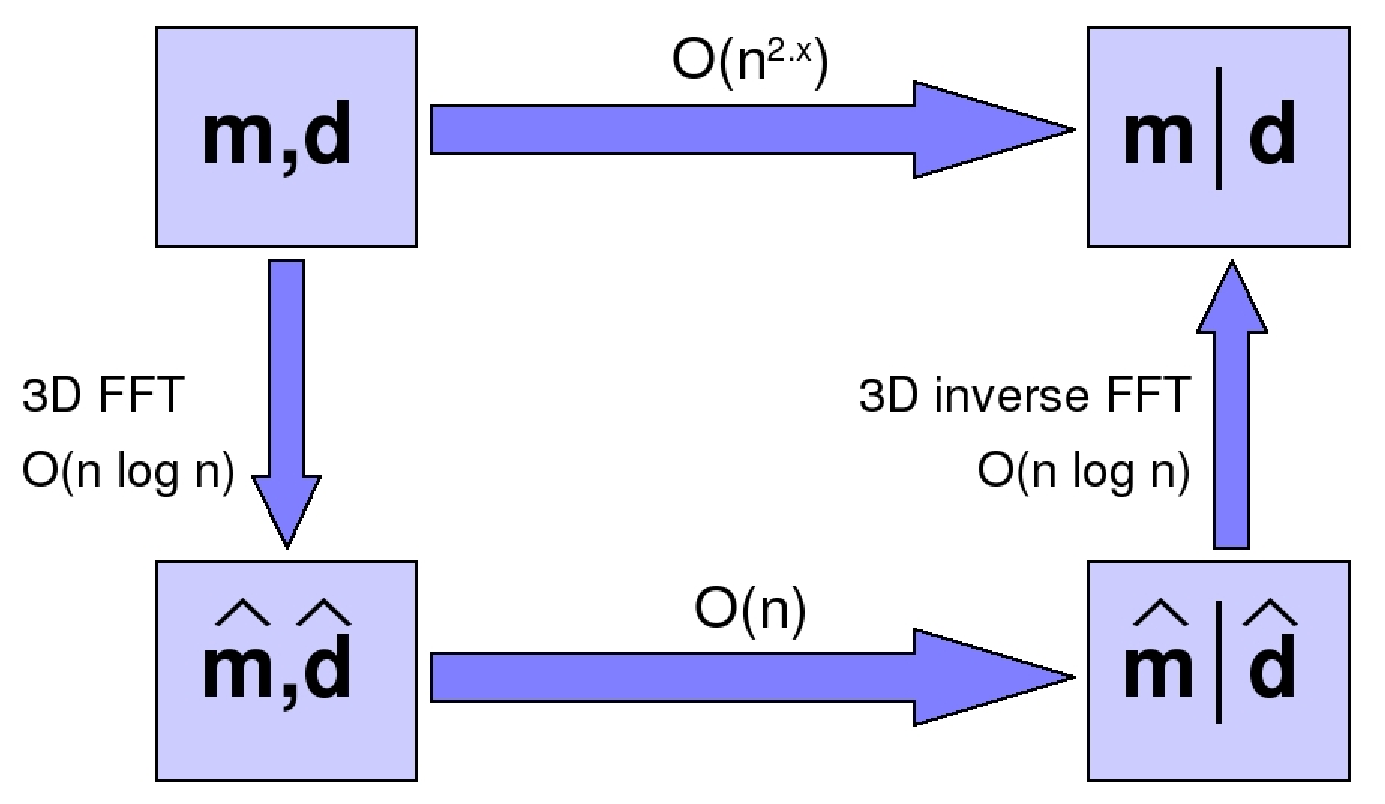
\includegraphics[width=.99\linewidth]{images/FFT_flowdiagram}
  \caption{The problem is transformed to the Fourier domain, solved
  in this domain, and back-transformed to time domain. This reduces
  the problem from a $\mathcal{O}(n^{2.x})$ to a $\mathcal{O}(n\log
  n)$ process.}
  \label{fig:FFT-flowdiagram}
\end{figure}

\noindent
interval is perfectly layered and the top and base surfaces follow
this layering exactly, the correlation ranges become
underestimated. As this may lead to numerical instabilities, a
parametric correlation function is typically used. In this case, the
same function is used for both correlations, and the correlation
function (type, ranges, and anisotropy angle) is given as input to the
program.

The error covariance matrix $\bSigma_{0,e}$ is also given as input
to the program. For an inversion system with two offsets $\theta_1$ and
$\theta_2$, the covariance matrix is
%
\begin{equation}
\bSigma_{0,e} =
\begin{bmatrix}
\sigma^2_{\theta_1}
& \sigma_{\theta_1}\sigma_{\theta_2}\nu_\theta(\phi)\\
\sigma_{\theta_1}\sigma_{\theta_2}\nu_\theta(\phi)
& \sigma^2_{\theta_1}\\
\end{bmatrix}
\end{equation}
%
\noindent
where $\sigma^2_{\theta_1}$ and $\sigma^2_{\theta_2}$ are the error
variances for offsets 1 and 2, respectively, and $\nu_\theta(\phi)$ is
an angular correlation function where $\phi=|\theta_2-\theta_1|$. The
variances and correlation function (type and range) are given as
\crava input.

The final part of the prior model, the error correlation function,
$\cet(\tau)$, consists of two parts. The first part gives the
correlation structure of the wavelet and is estimated by \crava, while
the other part is a white noise component and is given as program
input.

%\crava reads its input from a model file. In the model file the user
%specifies commands and parameters relevant for each command. There are
%commands available for specifying the seismic volumes, wavelets, and
%well data. The inversion region, the parts of the prior distribution
%not estimated by \crava, and the likelihood are also defined
%here. Finally, there are technical parameters that may be given, and
%commands for program output.

The model file used in the \crava run for the predicted parameters is
given in Appendix~\ref{sec:crava-model-file} for reference.
